\begin{surferPage}[30 نتوءاً]{منحنى بارت المسدس ذو 30 نتوءاً}
    A  بعد أن أنجز وولف بارت المنحنى المسدس مع اكبر عدد ممكن من المتفردات، $65$ (يمكن مراجعة هذا المنحنى في هذه الجاليريا) وبعد أن أنجز إثنان من طلابه في الدكتوراه منحنيات قياسية جديدة من درجة أعلى، أخذ يدرس عدد النتوءات الأقصى في منحنيات من درجة معينة.

     يمكن ملاءمة بناء منحنى بارت المسدس ذي $65$ متفرداً من نوع $A_1^{+-}$ (مخروط مزدوج) للنتوءات، فنحصل على $30$ نتوءاً:
    \[P_6 - \alpha \cdot K^3=0,\]
    حيث $P_6$ هي مستويات التناظر في مجسم عشروني وفي منحنى بارت المسدس الآخر على السواء، وحيث $K$ هي من جديد معادلة كرة الوحدة:
    \vspace*{-0.4em}
    \begin{center}
      \begin{tabular}{c@{\ }c@{\ }c@{\ }c}
        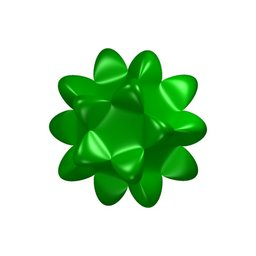
\includegraphics[height=1.2cm]{./../../common/images/barthsextic_30A2}
        &
        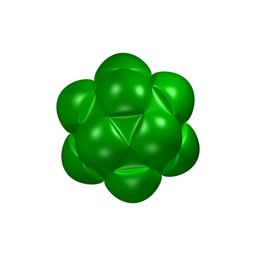
\includegraphics[height=1.2cm]{./../../common/images/barthsextic_30A2_3}
        &
        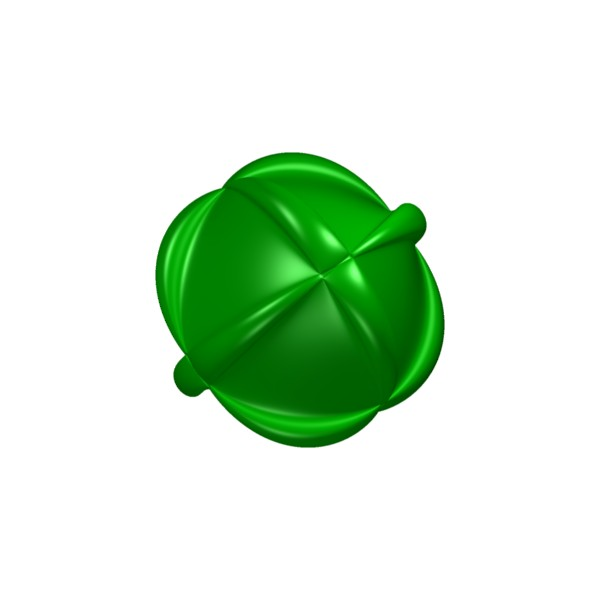
\includegraphics[height=1.2cm]{./../../common/images/barthsextic_30A2_5}
        &
        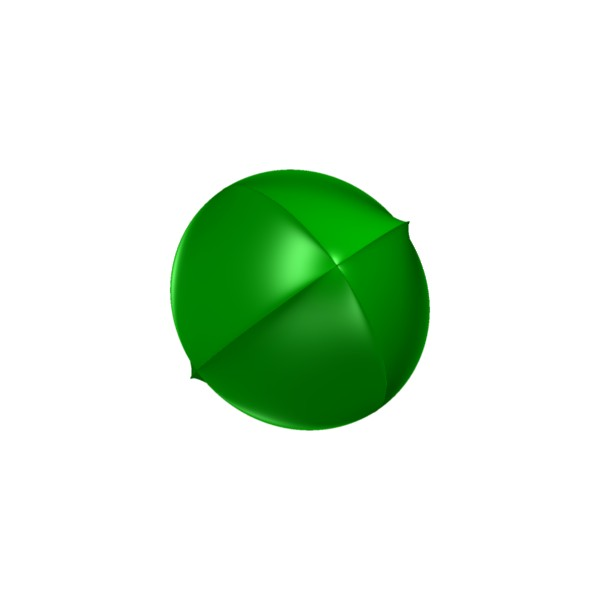
\includegraphics[height=1.2cm]{./../../common/images/barthsextic_30A2_6}
      \end{tabular}
    \end{center}
    \vspace*{-0.3em}
    هذا هو الرقم القياسي العالمي الحالي لأكبر عدد نتوءات حقيقية لمنحنى مسدس، أما عدد النتوءات المركبة فهو $36$.
\end{surferPage}
